\documentclass[12pt, a4papre]{article}
\usepackage[catalan]{babel}
\usepackage[unicode]{hyperref}
\usepackage{amsmath}
\usepackage{amssymb}
\usepackage{amsthm}
\usepackage{xifthen}
\usepackage{siunitx}
\usepackage{xcolor}
\usepackage{float}
\usepackage{listings}
\usepackage{setspace}
\usepackage{graphicx}
\usepackage{tikz,lipsum,lmodern}
\usepackage[most]{tcolorbox}
\usepackage{circuitikz}
\usepackage{indentfirst}
\usepackage{verbatimbox}
\usepackage[T1]{fontenc}
\usepackage{beramono}% monospaced font with bold variant
 \usepackage{tikz-timing}[2009/05/15]
\usepackage{listings}
\lstdefinelanguage{VHDL}{
   morekeywords={
     library,use,all,entity,is,port,in,out,end,architecture,of,
     begin,and
   },
   morecomment=[l]--
}
 
\usepackage{xcolor}
\colorlet{keyword}{blue!100!black!80}            
\colorlet{comment}{green!50!black!90}
\lstdefinestyle{vhdl}{
   language     = VHDL,
   basicstyle   = \ttfamily,
   keywordstyle = \color{keyword}\bfseries,
   commentstyle = \color{comment}
}

\graphicspath{ {./Imatges/} }


\newcommand{\norm}[1]{\lvert #1 \rvert}

\hypersetup{
    colorlinks = true,
    linkcolor = blue
}

\author{Daniel Vilardell\\
	   Igor Yuziv}
\title{Memoria practica 3}
\date{}

\begin{document}
	\maketitle
	\tableofcontents

	
	\newpage
	\section{Part 1}
	\subsection{Diseny Jerarquic}
	
	\subsection{ComptadorBCD}
	
		\begin{lstlisting}[style=vhdl, frame=single, basicstyle=\tiny]
		library ieee;
use ieee.std_logic_1164.all;
use ieee.std_logic_signed.all;

entity comptadorBCD is
	port (nrst, clk, ecnt : in std_logic;
		numx : out std_logic_vector(7 downto 0));
end comptadorBCD;

architecture compte of comptadorBCD is 
	signal unitats, desenes : std_logic_vector (3 downto 0);
	
begin 
	process(clk, nrst)
	begin
	    if nrst = '0' then desenes <= "0000";
			unitats <= "0000";
	    elsif clk' event and clk='1' then
		if ecnt = '1' then
		if desenes = "1001" and unitats = "1001" then desenes <= "0000";
			unitats <= "0000";
		elsif unitats = "1001" then desenes <= desenes +1;
			unitats <= "0000";
		else unitats <= unitats+1;
		end if;
	    end if;
	end if;
end process;
numx (7 downto 4) <= desenes;
numx (3 downto 0) <= unitats;

end compte;
		
		\end{lstlisting}
		
				
\begin{figure}[H]
		\begin{center}
		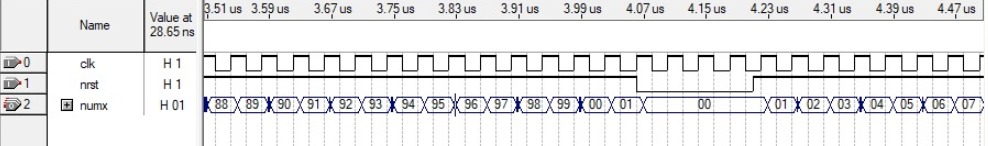
\includegraphics[width=130mm]{simulacioComptador.jpeg}
		\end{center}
	\end{figure}
\begin{figure}[H]
		\begin{center}
		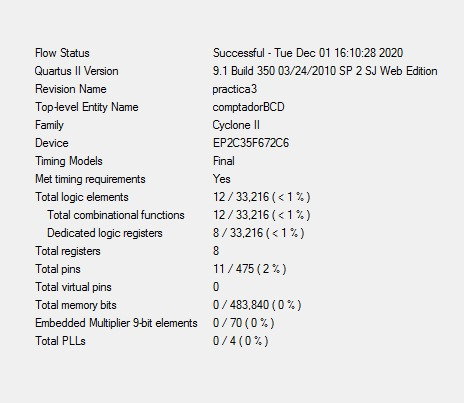
\includegraphics[width=130mm]{informeComptador.jpeg}
		\end{center}
	\end{figure}
	
	
\subsection{ComparadorBCD}


		
	\begin{lstlisting}[style=vhdl, frame=single, basicstyle=\tiny]
	library ieee;
use ieee.std_logic_1164.all;

entity comparadorBCD is 
	port (numx,num : in std_logic_vector (7 downto 0);
			ngtx,nltx,netx: out std_logic);
end comparadorBCD;

architecture comparador of comparadorBCD is 
	begin
	ngtx <= '1' when num > numx else '0';
	netx <= '1' when num = numx else '0';
	nltx <= '1' when num < numx else '0';
end comparador;
	
		\end{lstlisting}

\begin{figure}[H]
		\begin{center}
		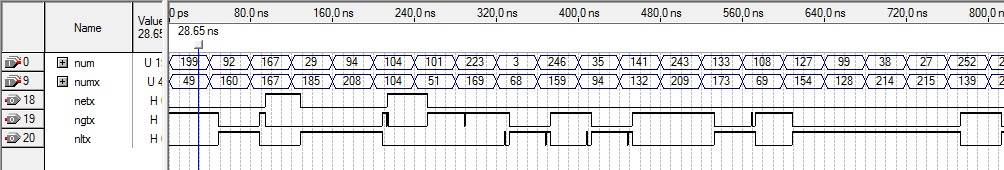
\includegraphics[width=130mm]{simulacioComparador.jpeg}
		\end{center}
	\end{figure}



\begin{figure}[H]
		\begin{center}
		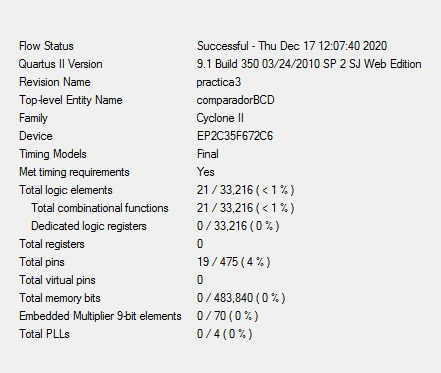
\includegraphics[width=130mm]{informeComparador.jpeg}
		\end{center}
	\end{figure}


\subsection{Control}
		
		\begin{lstlisting}[style=vhdl, frame=single, basicstyle=\tiny]
		
		library ieee;
use ieee.std_logic_1164.all;

entity control is
	port (nrst,clk,bcd,ast,coi,ngtx,netx,nltx : in std_logic;
		ecnt, eshft : out std_logic;
		led : out std_logic_vector(2 downto 0));
	end control;

architecture arcControl of control is 
	type maquina is (inicial, intro_data, mostrar_resultat);
	signal estat: maquina;
begin
	process(clk, nrst) begin
	if nrst = '0' then estat <= inicial;
	elsif (clk'event and clk ='1') then
	    case estat is 
	    when inicial => if ast = '1' then estat <= intro_data; end if;
	    when intro_data => if coi = '1' and ast = '0' then estat <= mostrar_resultat;
						   elsif ast = '1' then estat <= inicial; end if;
	    when mostrar_resultat => if ast = '1' then estat <= inicial;
				elsif netx = '1' then estat <= mostrar_resultat;
				elsif bcd = '1' then estat <= intro_data;
				end if;
	    end case;
	end if;
end process;

ecnt <= '1' when estat = inicial else '0';
eshft <= '1' when (estat = intro_data or estat = mostrar_resultat) and bcd = '1' else '0';
			
led <= "111" when estat = inicial 
    else "100" when estat = mostrar_resultat and nltx = '1' 
        and netx= '0' and ngtx = '0'
    else "010" when estat = mostrar_resultat and netx = '1' 
    	and nltx = '0' and ngtx = '0'
    else "001" when estat = mostrar_resultat and ngtx = '1' 
    	and nltx = '0' and netx = '0'
    else "000";
end arcControl;
		
		\end{lstlisting}
		
		Aqui falte simulacio de Control 

	
	
	\begin{figure}[H]
		\begin{center}
		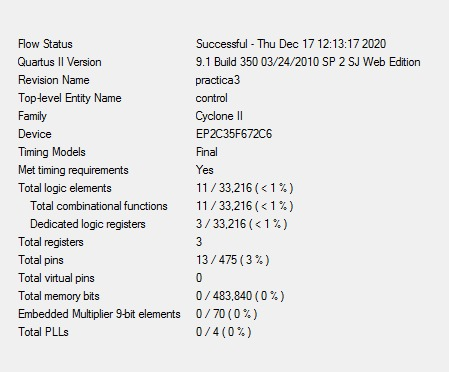
\includegraphics[width=130mm]{informeControl.jpeg}
		\end{center}
	\end{figure}	
		
		
\subsection{Registres}
		\begin{lstlisting}[style=vhdl, frame=single, basicstyle=\tiny]

library ieee;
use ieee.std_logic_1164.all;

entity regs_v is
	port(clk, nrst, intro : in std_logic;
		 keycode : in std_logic_vector(3 downto 0);
		 opA, opB: out std_logic_vector(3 downto 0));
end regs_v;

architecture arq of regs_v is
signal a, b : std_logic_vector(3 downto 0);
begin
process (clk, nrst)
begin 
	if(nrst = '0') then a <= "0000"; b <= "0000";
	elsif(nrst='1') and (clk'event and clk = '1') and (intro = '1') then
			b <= a;
			a <= keycode;
	end if;
end process;
opA <= a;
opB <= b;

end arq;

		\end{lstlisting}
		
			\begin{figure}[H]
		\begin{center}
		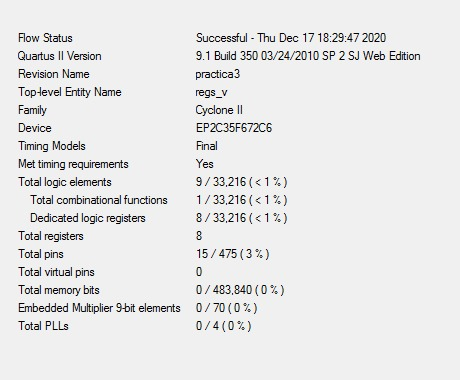
\includegraphics[width=130mm]{informeRegs.jpeg}
		\end{center}
	\end{figure}	

		
		

\subsection{keygroup}
		\begin{lstlisting}[style=vhdl, frame=single, basicstyle=\tiny]
	library ieee;
use ieee.std_logic_1164.all;

entity keygroup_v is
	port(nkey : in std_logic;
		k : in std_logic_vector(3 downto 0);
		bcd, ast, coi : out std_logic);
end keygroup_v;

architecture arq of keygroup_v is
begin
process (nkey, k)
begin
	if (nkey = '0' and (k = "0000" or k = "0001" or k = "0010" or
						k = "0011" or k = "0100" or k = "0101" or
						k = "0110" or k = "0111" or k = "1000" or
						k = "1001")) then bcd <= '1'; ast <= '0'; coi <= '0';
	elsif(nkey = '0' and k = "1110")
			then bcd <= '0'; ast <= '1'; coi <= '0';
	elsif(nkey = '0' and k = "1111")
			then bcd <= '0'; ast <= '0'; coi <= '1';
	elsif(nkey = '1') then bcd <= '0'; ast <= '0'; coi <= '0';
	end if;
end process;
end arq;
		\end{lstlisting}
		
			\begin{figure}[H]
		\begin{center}
		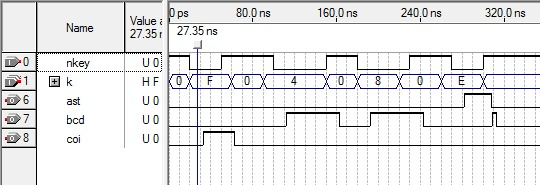
\includegraphics[width=130mm]{simulaciokeygroup.jpeg}
		\end{center}
	\end{figure}	
	
	
	
			\begin{figure}[H]
		\begin{center}
		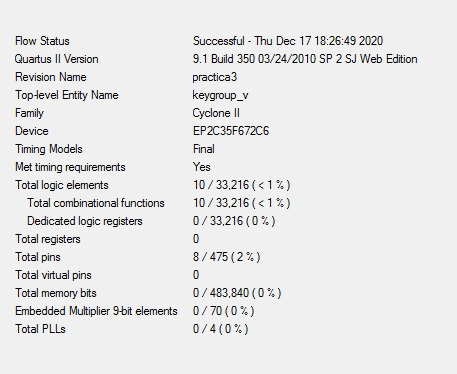
\includegraphics[width=130mm]{informeKeygroup.jpeg}
		\end{center}
	\end{figure}	
	
	
	\subsection{Joc}
	
	
				\begin{figure}[H]
		\begin{center}
		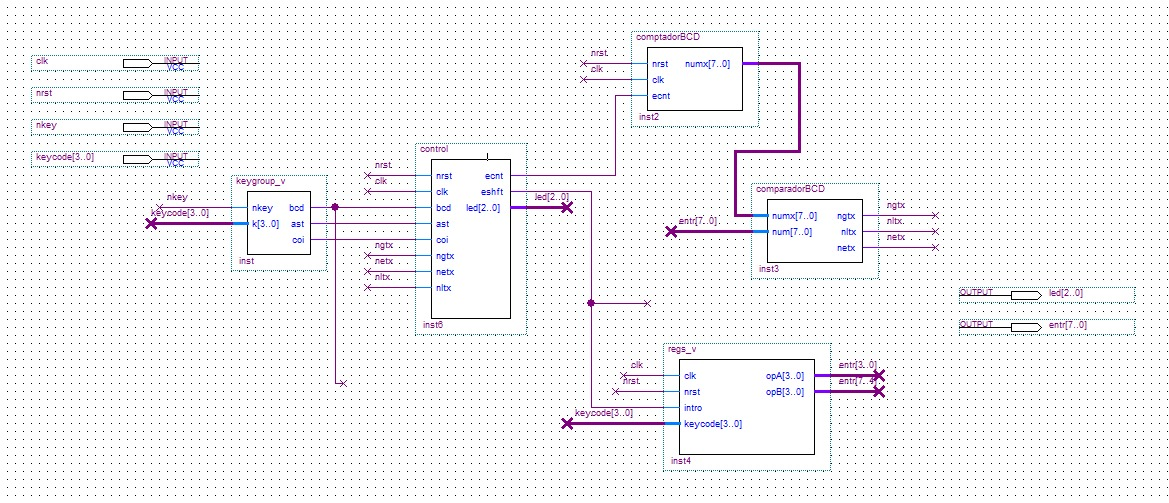
\includegraphics[width=130mm]{joc.jpeg}
		\end{center}
	\end{figure}	
			\begin{figure}[H]
		\begin{center}
		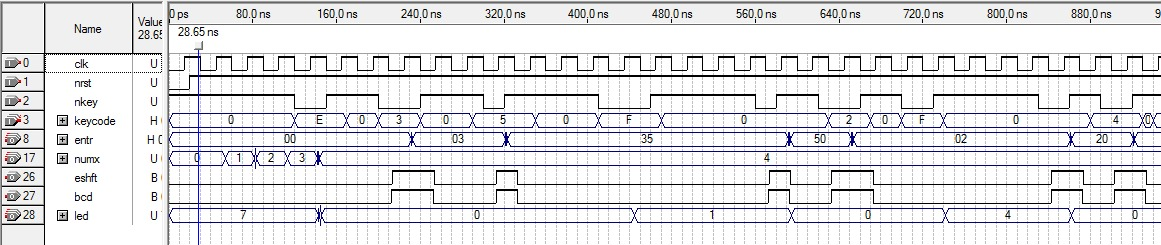
\includegraphics[width=130mm]{simulacioJoc.jpeg}
		\end{center}
	\end{figure}	
			\begin{figure}[H]
		\begin{center}
		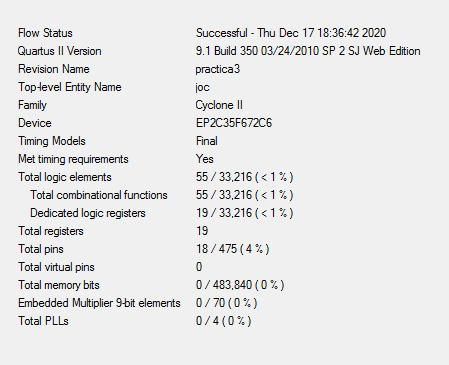
\includegraphics[width=130mm]{informeJoc.jpeg}
		\end{center}
	\end{figure}	

		
	\subsection{Joc Placa}
	
	
	
				\begin{figure}[H]
		\begin{center}
		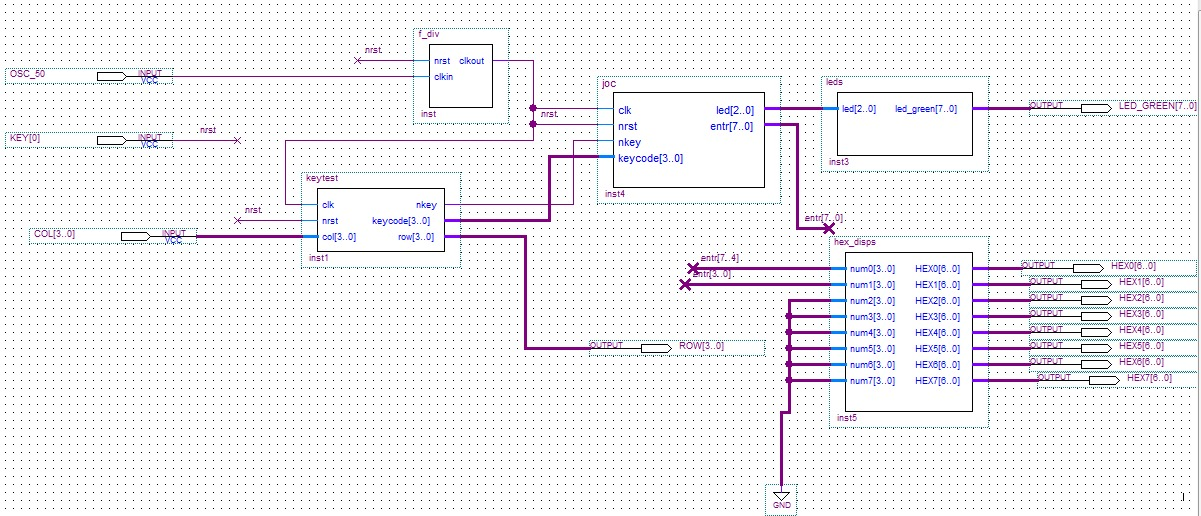
\includegraphics[width=130mm]{jocPlaca.jpeg}
		\end{center}
	\end{figure}	



\section{Part Extra}

\subsection{ComptadorBCD Extra}

	\begin{lstlisting}[style=vhdl, frame=single, basicstyle=\tiny]

library ieee;
use ieee.std_logic_1164.all;
use ieee.std_logic_signed.all;

entity comptadorBCD_extra is
	port (nrst, clk, ecnt : in std_logic;
		numx : out std_logic_vector(11 downto 0));
end comptadorBCD_extra;

architecture compte of comptadorBCD_extra is 
	signal unitats, desenes, centenes : std_logic_vector (3 downto 0);
	
begin 
	process(clk, nrst)
	begin
	    if nrst = '0' then desenes <= "0000";
			unitats <= "0000"; centenes <= "0000";
	    elsif clk' event and clk='1' then
		if ecnt = '1' then
		if desenes = "1001" and unitats = "1001" and centenes = "1001" 
			then desenes <= "0000"; unitats <= "0000"; centenes <= "0000";
		elsif desenes = "1001" and unitats = "1001" then centenes <= centenes + 1;
			desenes <= "0000"; unitats <= "0000";
		elsif unitats = "1001" then desenes <= desenes + 1;
			unitats <= "0000";
		else unitats <= unitats+1;
		end if;
	    end if;
	end if;
end process;
numx (11 downto 8) <= centenes;
numx (7 downto 4) <= desenes;
numx (3 downto 0) <= unitats;

end compte;

		\end{lstlisting}
		
				\begin{figure}[H]
		\begin{center}
		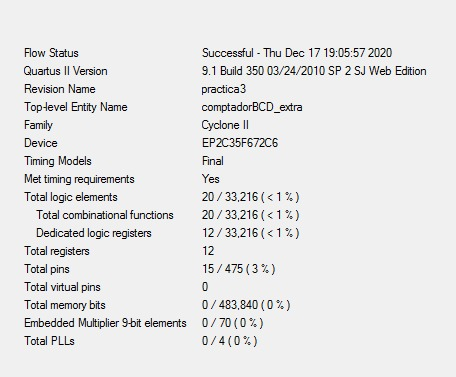
\includegraphics[width=130mm]{informeComptadorBCDextra.jpeg}
		\end{center}
	\end{figure}	
		

\subsection{Registres Extra}

	\begin{lstlisting}[style=vhdl, frame=single, basicstyle=\tiny]
	library ieee;
use ieee.std_logic_1164.all;

entity regs_extra is
	port(clk, nrst, intro : in std_logic;
		 keycode : in std_logic_vector(3 downto 0);
		 opA, opB, opC: out std_logic_vector(3 downto 0));
end regs_extra;

architecture arq of regs_extra is
signal a, b, c : std_logic_vector(3 downto 0);
begin
process (clk, nrst)
begin 
	if(nrst = '0') then a <= "0000"; b <= "0000"; c <= "0000";
	elsif(nrst='1') and (clk'event and clk = '1') and (intro = '1') then
			c <= b;
			b <= a;
			a <= keycode;
	end if;
end process;
opA <= a;
opB <= b;
opC <= c;

end arq;
	
			\end{lstlisting}
			
						\begin{figure}[H]
		\begin{center}
		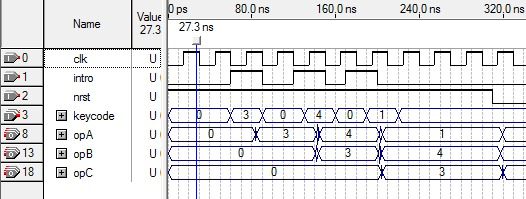
\includegraphics[width=130mm]{simularioRegistreExtra.jpeg}
		\end{center}
	\end{figure}	
	
					\begin{figure}[H]
		\begin{center}
		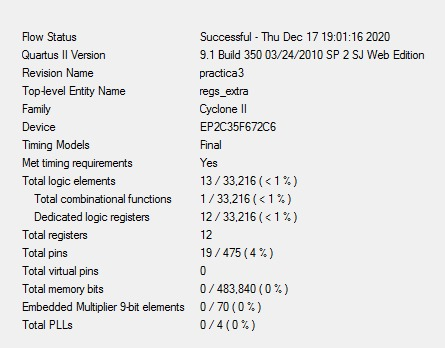
\includegraphics[width=130mm]{informeRegsExtra.jpeg}
		\end{center}
	\end{figure}	
	
			
			

\subsection{Keygroup Extra}


	\begin{lstlisting}[style=vhdl, frame=single, basicstyle=\tiny]

library ieee;
use ieee.std_logic_1164.all;

entity keygroup_extra is
	port(nkey : in std_logic;
		k : in std_logic_vector(3 downto 0);
		bcd, ast, coi, A, B : out std_logic);
end keygroup_extra;

architecture arq of keygroup_extra is
begin
process (nkey, k)
begin
	if (nkey = '0' and (k = "0000" or k = "0001" or k = "0010" or
						k = "0011" or k = "0100" or k = "0101" or
						k = "0110" or k = "0111" or k = "1000" or
						k = "1001")) then bcd <= '1'; ast <= '0'; coi <= '0'; A <= '0'; B <= '0';
	elsif(nkey = '0' and k = "1010") then bcd <= '0'; ast <= '0'; coi <= '0'; A <= '1'; B <= '0';
	elsif(nkey = '0' and k = "1011") then bcd <= '0'; ast <= '0'; coi <= '0'; A <= '0'; B <= '1';
	elsif(nkey = '0' and k = "1110") then bcd <= '0'; ast <= '1'; coi <= '0'; A <= '0'; B <= '0';
	elsif(nkey = '0' and k = "1111") then bcd <= '0'; ast <= '0'; coi <= '1'; A <= '0'; B <= '0';
	elsif(nkey = '1') then bcd <= '0'; ast <= '0'; coi <= '0'; A <= '0'; B <= '0';
	else bcd <= '0'; ast <= '0'; coi <= '0'; A <= '0'; B <= '0';
	end if;
end process;
end arq;


			\end{lstlisting}
			
			
						\begin{figure}[H]
		\begin{center}
		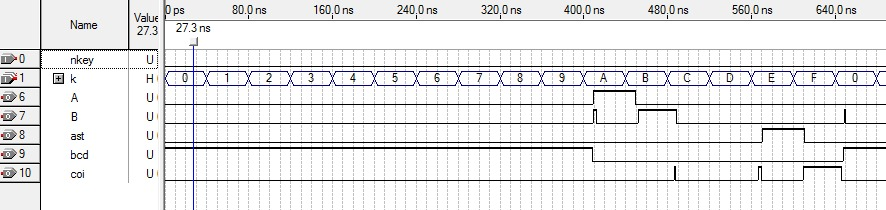
\includegraphics[width=130mm]{simulacioKeyGroupExtra.jpeg}
		\end{center}
	\end{figure}	
		\begin{figure}[H]
			
				\begin{center}
		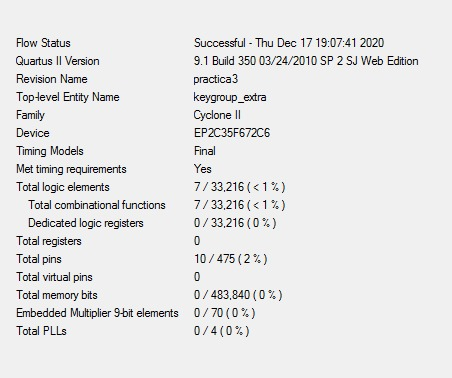
\includegraphics[width=130mm]{informeKeyGroupExtra.jpeg}
		\end{center}
	\end{figure}	
			
			
\subsection{Control Extra}

	\begin{lstlisting}[style=vhdl, frame=single, basicstyle=\tiny]

library ieee;
use ieee.std_logic_1164.all;
use ieee.std_logic_unsigned.all;

entity control_extra is
	port (nrst,clk,bcd,ast,coi,A,B,ngtx,netx,nltx : in std_logic;
		ecnt, eshft : out std_logic;
		led : out std_logic_vector(2 downto 0);
		tot : out std_logic_vector(3 downto 0));
	end control_extra;

architecture arcControl of control_extra is 
	type maquina is (inicial, intro_data, mostrar_resultat, trampa_A, trampa_B);
	signal estat: maquina;
	signal t : std_logic_vector(3 downto 0);
begin
	process(clk, nrst) begin
	if nrst = '0' then estat <= inicial;
	elsif (clk'event and clk ='1') then
	    case estat is 
	    when inicial => if ast = '1' then estat <= intro_data; end if;
	    when intro_data => if coi = '1' and ast = '0' then estat <= mostrar_resultat;
						   elsif ast = '1' then estat <= inicial;
						   elsif A = '1' then estat <= trampa_A;
						   elsif B = '1' then estat <= trampa_B; end if;
	    when mostrar_resultat => if ast = '1' then estat <= inicial;
				elsif bcd = '1' then estat <= intro_data;
				elsif A = '1' then estat <= trampa_A;
				elsif B = '1' then estat <= trampa_B;
				end if;
		when trampa_A => if ast = '1' then estat <= inicial;
				elsif bcd = '1' then estat <= intro_data;
				elsif B = '1' then estat <= trampa_B;
				end if;
		when trampa_B => if ast = '1' then estat <= inicial;
				elsif bcd = '1' then estat <= intro_data;
				elsif A = '1' then estat <= trampa_A;
				end if;
		end case;
		if(netx = '1' and estat = intro_data) then t <= t + 1; estat <= inicial; end if;
	end if;
end process;
tot <= t;

ecnt <= '1' when estat = inicial else '0';
eshft <= '1' when (estat = intro_data or estat = mostrar_resultat) and bcd = '1' else '0';
			
led <= "111" when estat = inicial 
    else "100" when estat = mostrar_resultat and nltx = '1' 
        and netx= '0' and ngtx = '0'
    else "010" when estat = mostrar_resultat and netx = '1' 
    	and nltx = '0' and ngtx = '0'
    else "001" when estat = mostrar_resultat and ngtx = '1' 
    	and nltx = '0' and netx = '0'
    else "110" when estat = trampa_A
    else "011" when estat = trampa_B
    else "000";
end arcControl;

			\end{lstlisting}
			
			
			
				\begin{figure}[H]
			
				\begin{center}
		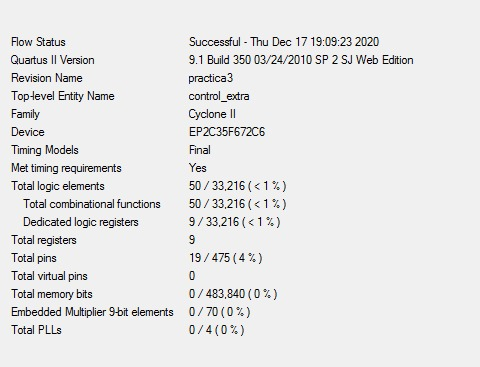
\includegraphics[width=130mm]{informeControlExtra.jpeg}
		\end{center}
	\end{figure}	
			
\subsection{Trampes}
	\begin{lstlisting}[style=vhdl, frame=single, basicstyle=\tiny]

library ieee;
use ieee.std_logic_1164.all;

entity trampes is
	port(tr : in std_logic_vector(2 downto 0);
		 num: in std_logic_vector(11 downto 0);
		 mostra: out std_logic_vector(3 downto 0));
end trampes;

architecture arq of trampes is
begin
process (tr)
begin
	if tr = "110" then mostra <= num(3 downto 0);
	elsif tr = "011" then mostra <= num(7 downto 4);
	else mostra <= "0000";
	end if;
end process;
end arq;



			\end{lstlisting}
			
			\begin{figure}[H]
			
				\begin{center}
		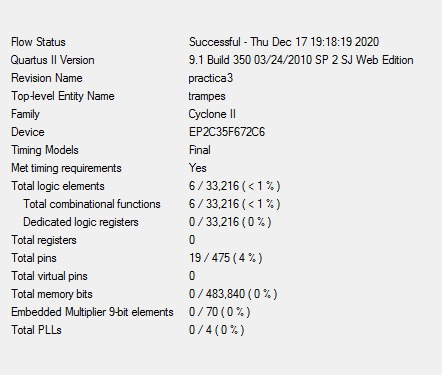
\includegraphics[width=130mm]{informeTrampes.jpeg}
		\end{center}
	\end{figure}	

			
			
\subsection{Leds}

	\begin{lstlisting}[style=vhdl, frame=single, basicstyle=\tiny]
	library ieee;
use ieee.std_logic_1164.all;

entity led_extra is
	port(led: in std_logic_vector(2 downto 0);
		 num : in std_logic_vector(3 downto 0);
		 led_green : out std_logic_vector(7 downto 0);
		 led_level : out std_logic_vector(7 downto 0));
end led_extra;

architecture arq of led_extra is
begin
	led_green <= "11111111" when led = "111" else
				 "11110000" when led = "100" else
				 "00001111" when led = "001" else
				 "00111100" when led = "010" else
				 "00000000" when led = "000" else
				 "01010101" when led = "110" else
				 "10101010" when led = "011";
	led_level <= "00000000" when num = "0000" else
				 "10000000" when num = "0001" else
				 "11000000" when num = "0010" else
				 "11100000" when num = "0011" else
				 "11110000" when num = "0100" else
				 "11111000" when num = "0101" else
				 "11111100" when num = "0110" else
				 "11111110" when num = "0111" else
				 "11111111" when num = "1000";
				 
end arq;
	\end{lstlisting}
	

	
			\begin{figure}[H]
			
				\begin{center}
		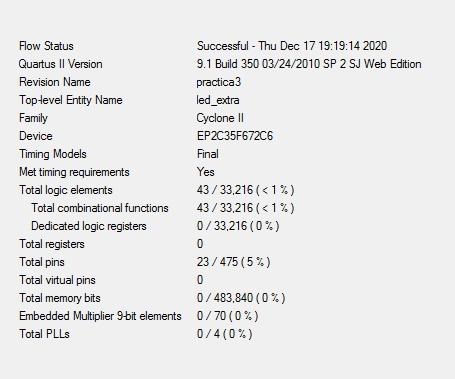
\includegraphics[width=130mm]{informeLeds.jpeg}
		\end{center}
	\end{figure}
	
\subsection{Temporitzador}


\begin{lstlisting}[style=vhdl, frame=single, basicstyle=\tiny]
	library ieee;
use ieee.std_logic_1164.all;
use ieee.std_logic_signed.all;

entity temporitzador is
	port (nrst, clk, ecnt : in std_logic;
		numx : out std_logic_vector(7 downto 0));
end temporitzador;

architecture compte of temporitzador is 
	signal unitats, desenes : std_logic_vector (3 downto 0);
	
begin 
	process(clk, nrst)
	begin
	    if nrst = '0' then desenes <= "1001";
			unitats <= "1001";
	    elsif clk' event and clk='1' then
		if ecnt = '1' then
		if desenes = "0000" and unitats = "0000" then desenes <= "0000";
			unitats <= "0000";
		elsif unitats = "0000" then desenes <= desenes -1;
			unitats <= "1001";
		else unitats <= unitats-1;
		end if;
	    end if;
	end if;
end process;
numx (7 downto 4) <= desenes;
numx (3 downto 0) <= unitats;

end compte;
	\end{lstlisting}
	
	
			\begin{figure}[H]
			
				\begin{center}
		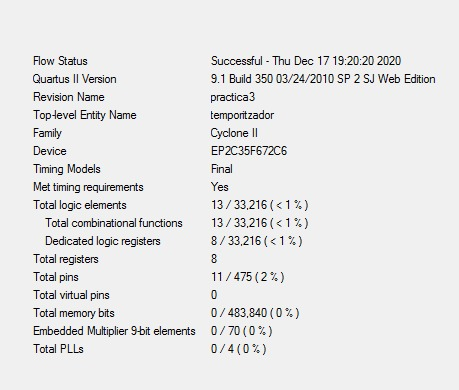
\includegraphics[width=130mm]{informeTemporitzador.jpeg}
		\end{center}
	\end{figure}
	
	
\subsection{Slow Timer}
\begin{lstlisting}[style=vhdl, frame=single, basicstyle=\tiny]
	-- Frequency divider by M
-- D = output duty cycle in %
-- version DD-1.0 - march 2011

library ieee;
use ieee.std_logic_1164.all;

entity slow_timer is 
  port( nrst,clkin : in std_logic; 
        clkout : out std_logic );
end slow_timer;

architecture dni of slow_timer is
constant M : integer :=750;
constant D : integer :=50;
constant n : integer :=D*M/100;
signal q : integer range 0 to M-1;
begin
  process(clkin,nrst) begin
     if nrst='0' then clkout <= '0'; q <= 0;
     elsif clkin'event and clkin='1' then 
         if q < M-1 then q <= q+1; 
            else q <= 0; end if;
         if q < n then clkout <= '1';
            else clkout <= '0'; end if;
     end if;
  end process;
end dni;
	\end{lstlisting}
	

	
		\begin{figure}[H]
			
				\begin{center}
		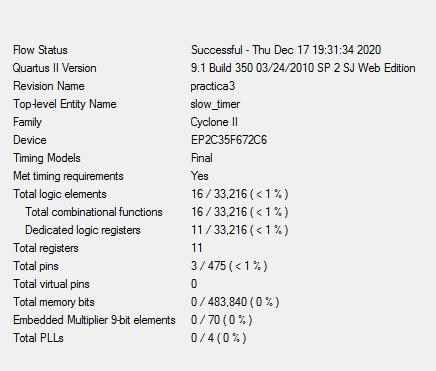
\includegraphics[width=130mm]{informeSlowTimer.jpeg}
		\end{center}
	\end{figure}
\subsection{Joc Extra}


\begin{figure}[H]
			
				\begin{center}
		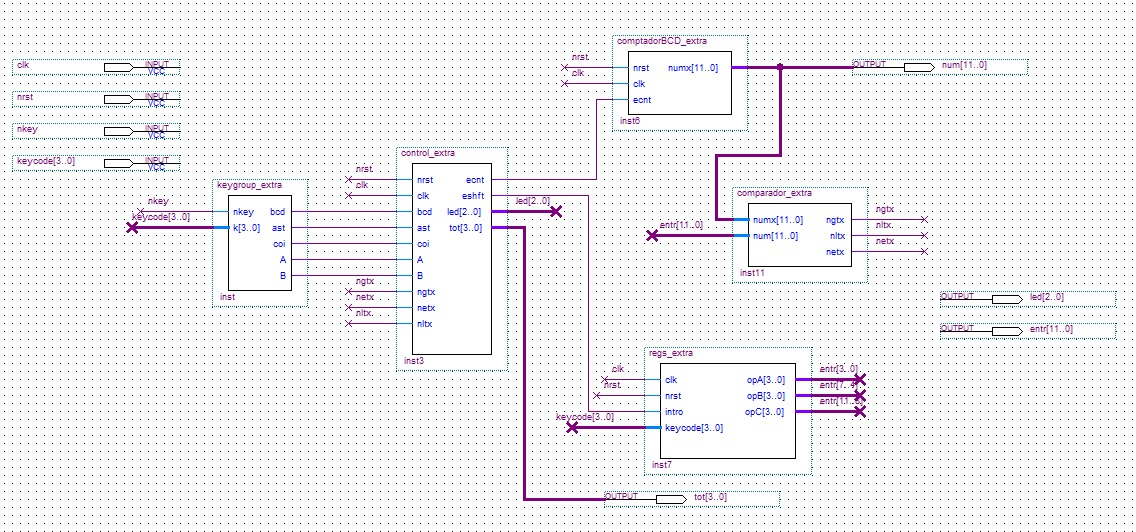
\includegraphics[width=130mm]{jocExtra.jpeg}
		\end{center}
	\end{figure}
	
	\begin{figure}[H]
	
				\begin{center}
		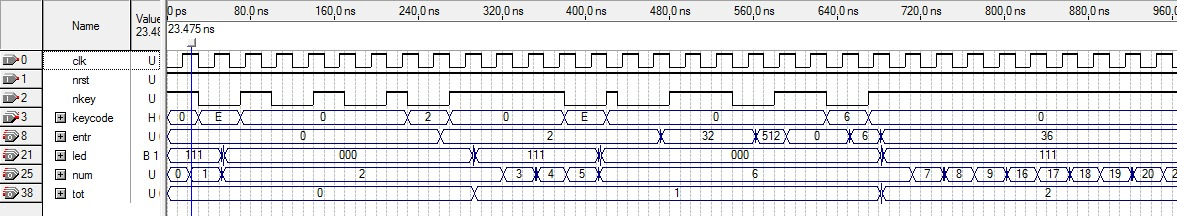
\includegraphics[width=130mm]{SimulacioJocExtra.jpeg}
		\end{center}
	\end{figure}
	
	
	\begin{figure}[H]
	
				\begin{center}
		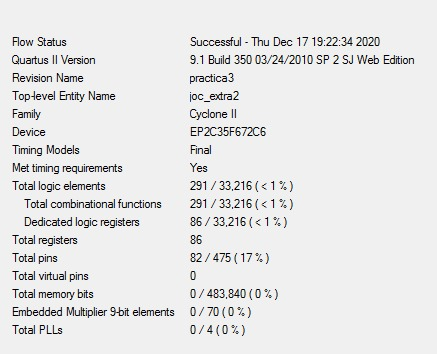
\includegraphics[width=130mm]{informeJocExtra.jpeg}
		\end{center}
	\end{figure}
	

\subsection{Joc Extra Placa}

	\begin{figure}[H]
	
				\begin{center}
		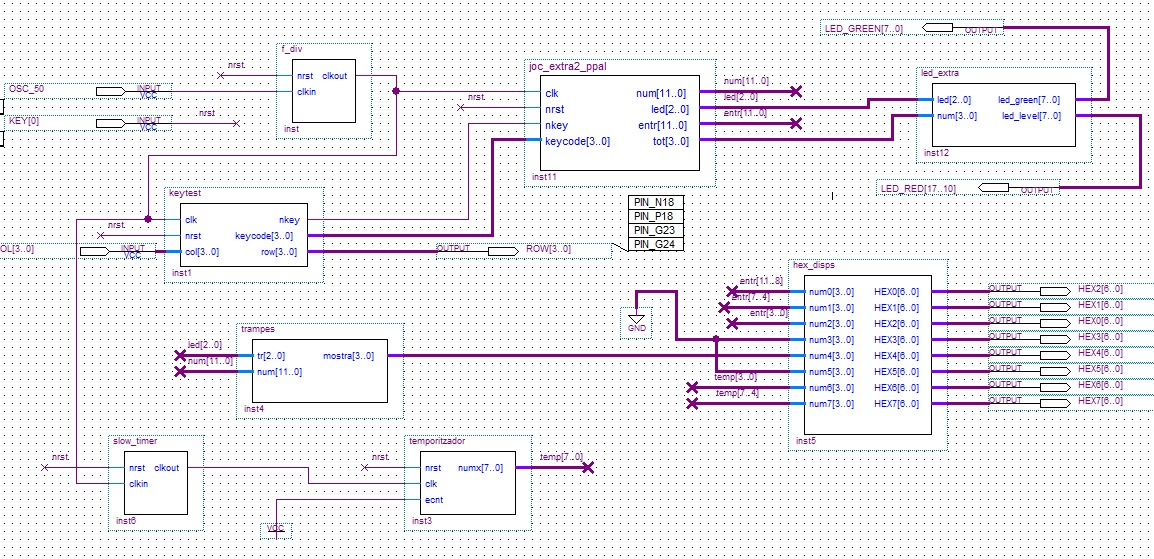
\includegraphics[width=130mm]{JocExtraPlaca.jpeg}
		\end{center}
	\end{figure}





	
	
\end{document}